\section{Ice: the Antarctic pairs of nisarErrors}
\label{sec:antarctica}

\citet{joughin2026nisarerrors} compared the ionosphere corrections of NISAR's PR products with those of GrIMP, the
processing that turns NISAR interferograms into ice-velocity maps \citep{joughin2018grimp}, on two pairs over Greenland
and two over Antarctica. Over Greenland their main finding is a carrier error. ISCE3 registers the second date to the
ionosphere's azimuth shift, and the Doppler carrier turns that shift into a phase that scales with frequency. No
split-spectrum form removes it, and it is not considered here. Over Antarctica, on track 94 descending, frame 129
(80.2--82.9$^\circ$S, 13--33$^\circ$W, grounded ice upstream of the Filchner Ice Shelf), they found two things.
\begin{itemize}
  \item The RUNW's screen is about 40\,rad off over part of the second of its two connected components, between the
        component boundary and a glacier's shear margin.
  \item The unwrapped phase is split between the components. GrIMP fixes the split from its velocity map, at $-7$
        cycles in both pairs.
\end{itemize}
Against GrIMP's own velocity synthetic, the RUNW's corrected phase leaves a residual of 21.5 and 21.9\,rad (robust 26.8
and 26.6), and GrIMP's leaves 2.61 and 2.59 (2.20 and 2.00).
\authnote{\citet{joughin2026nisarerrors} is a public draft in a code repository; check with its author before citing
it.}

For an interferogram, a glacier's shear margin is what a strike-slip rupture is: a steep step in the non-dispersive
phase, decorrelated over kilometres, that the unwrapper may not cross. The products were made with the recipe of
Section~\ref{sec:nisar} (ISCE3 0.25.16, \texttt{main\_diff\_ms\_band}, \texttt{unwrap\_correction: True}, read from
their run configuration). These pairs therefore test Section~\ref{sec:theory}'s account on data that hold no
earthquake, and the range offsets give an independent check.

\subsection{Data and processing}
The pairs are 19--31 August and 31 August -- 12 September 2026, in NISAR's 40\,+\,5\,MHz mode, HH. They go through the
pipeline of Section~\ref{sec:nisar} with three differences.
\begin{itemize}
  \item The registration field is the GUNW's own pixel offsets, the field ISCE3 applied, plus the first date's TEC and
        solid-earth-tide shift (Appendix~\ref{app:registration}). Gross outliers, more than 5\,m from their 600\,m
        neighbourhood, are removed first.
  \item The main band is the product's own unwrapped phase, so that the comparison isolates the screen. Fast ice puts
        several fringes into a 240\,m cell, so the cells take it out of every pixel before the sums
        (Section~\ref{sec:pixel}). Its sign was checked on the 20\,km box where it changes fastest: the cells' median
        coherence there is 0.55 with it taken out, 0.49 without it, and 0.31 with its sign flipped (pair 1).
  \item There is no fault zone to exclude.
\end{itemize}
Our screen is made three ways: with the main band's integers as delivered, from the main component alone, and with the
other component re-tied to it by the side band (Section~\ref{sec:sbtie}). The product's screen is binned onto the same
cells. The estimators of Section~\ref{sec:synthetic} also run on these cells, with the absolute cell phases rebuilt from
the model's cell mean. Their \texttt{ours} reproduces the tied screen to 0.002\,rad rms.

\begin{table}[p]
\centering
\caption{The Antarctic pairs (track 94 descending, frame 129).
\emph{The product's screen minus ours}, cell by cell: component 1's offset in main-band cycles (3.21\,rad), the block's
in cycles of the double difference (72.96\,rad), and what is left.
\emph{The split of component 1}, read three ways in the same 17 windows along the boundary, beside GrIMP's fix, and the
non-dispersive step across the gap there.
\emph{Over the tributary's trunk}: the plateau left after the integers, what ISCE3's correction passes add there on our
cells, and the leak (slope, and $r$ in brackets, of the screen's 15\,km high-pass on the non-dispersive phase's) with
the cells within 5\,km of either integer step left out.
\emph{The offsets' ionosphere} minus each screen: where the screens differ, $(\phiA - k\rho_\mathrm{off})$ smoothed over
3\,km and calibrated on ours; over the frame, $(\phiA - k\rho_\mathrm{off})/2$ uncalibrated, both smoothed over 6\,km, a
median and a plane removed per screen.
\emph{nisarErrors' residual metric} against an ITS\_LIVE synthetic, on slow grounded ice ($<$50\,m/yr).
\emph{Pair 1 minus pair 2}: the corrected phases' difference, a median and a plane removed, on the pixels coherent in
both.}
\label{tab:antarctica}
\small
\setlength{\tabcolsep}{4pt}
\begin{tabular}{lrr}
\toprule
 & pair 1 & pair 2 \\
 & 19--31 Aug & 31 Aug--12 Sep \\
\midrule
\multicolumn{3}{l}{\emph{The product's screen minus ours}} \\
component 1, in main-band cycles & 9.013 & 8.004 \\
the block, in double-difference cycles & 1.0006 & 0.9995 \\
\quad its area (km$^2$) & 11\,980 & 11\,304 \\
left after the integers: robust sd (rad) & 0.13 & 0.13 \\
\quad area beyond 3\,rad (km$^2$) & 5\,400 & 5\,078 \\
\addlinespace
\multicolumn{3}{l}{\emph{The split of component 1, in main-band cycles}} \\
side band (median of 17 windows) & 8.95 & 7.97 \\
range offsets, $\phi_A - k\rho_\mathrm{off}$: the GUNW's & 8.90 & 7.96 \\
\quad ours, a gross-outlier cull only & 9.06 & 8.15 \\
ITS\_LIVE, slow ice within 20\,km & 8.01 & -- \\
GrIMP's fix \citep{joughin2026nisarerrors} & 7 & 7 \\
non-dispersive step across the gap (rad) & 74--188 & 80--188 \\
\addlinespace
\multicolumn{3}{l}{\emph{Over the tributary's trunk, 5--20\,km outside the block}} \\
product $-$ ours $-$ integers (rad) & 6.50 & 5.44 \\
\quad in main-band cycles & 2.03 & 1.70 \\
ISCE3's passes on our cells (rad) & 3.60 & 3.52 \\
leak away from the integer steps: product & -0.066 (-0.65) & -0.066 (-0.67) \\
\quad ours & 0.002 (0.09) & 0.001 (0.03) \\
\addlinespace
\multicolumn{3}{l}{\emph{The offsets' ionosphere minus each screen (rad)}} \\
product above ours by $>$3\,rad: minus ours / minus product & -0.28 / -5.60 & -0.32 / -4.91 \\
product below ours by $>$3\,rad: minus ours / minus product & +0.34 / +3.47 & +0.27 / +3.01 \\
over the frame, rms (6\,km): product / repaired / ours & 18.85 / 1.29 / 0.63 & 18.85 / 1.21 / 0.68 \\
\addlinespace
\multicolumn{3}{l}{\emph{Phase minus an ITS\_LIVE synthetic, slow ice: $\sigma$ / robust $\sigma$ (rad)}} \\
uncorrected & 3.50 / 3.15 & 2.09 / 1.69 \\
the product's screen & 15.19 / 14.24 & 15.05 / 14.08 \\
the product's, integers repaired & 4.04 / 1.36 & 3.97 / 1.44 \\
ours & 1.84 / 1.22 & 1.84 / 1.21 \\
\addlinespace
\multicolumn{3}{l}{\emph{Pair 1 minus pair 2, a median and plane out: $\sigma$ / robust $\sigma$ (rad)}} \\
uncorrected & \multicolumn{2}{c}{3.94 / 4.13} \\
the product's screen & \multicolumn{2}{c}{1.30 / 0.99} \\
the product's, integers repaired & \multicolumn{2}{c}{2.70 / 0.86} \\
ours & \multicolumn{2}{c}{1.02 / 0.81} \\
\bottomrule
\end{tabular}

\end{table}

\begin{figure}[p]
\centering
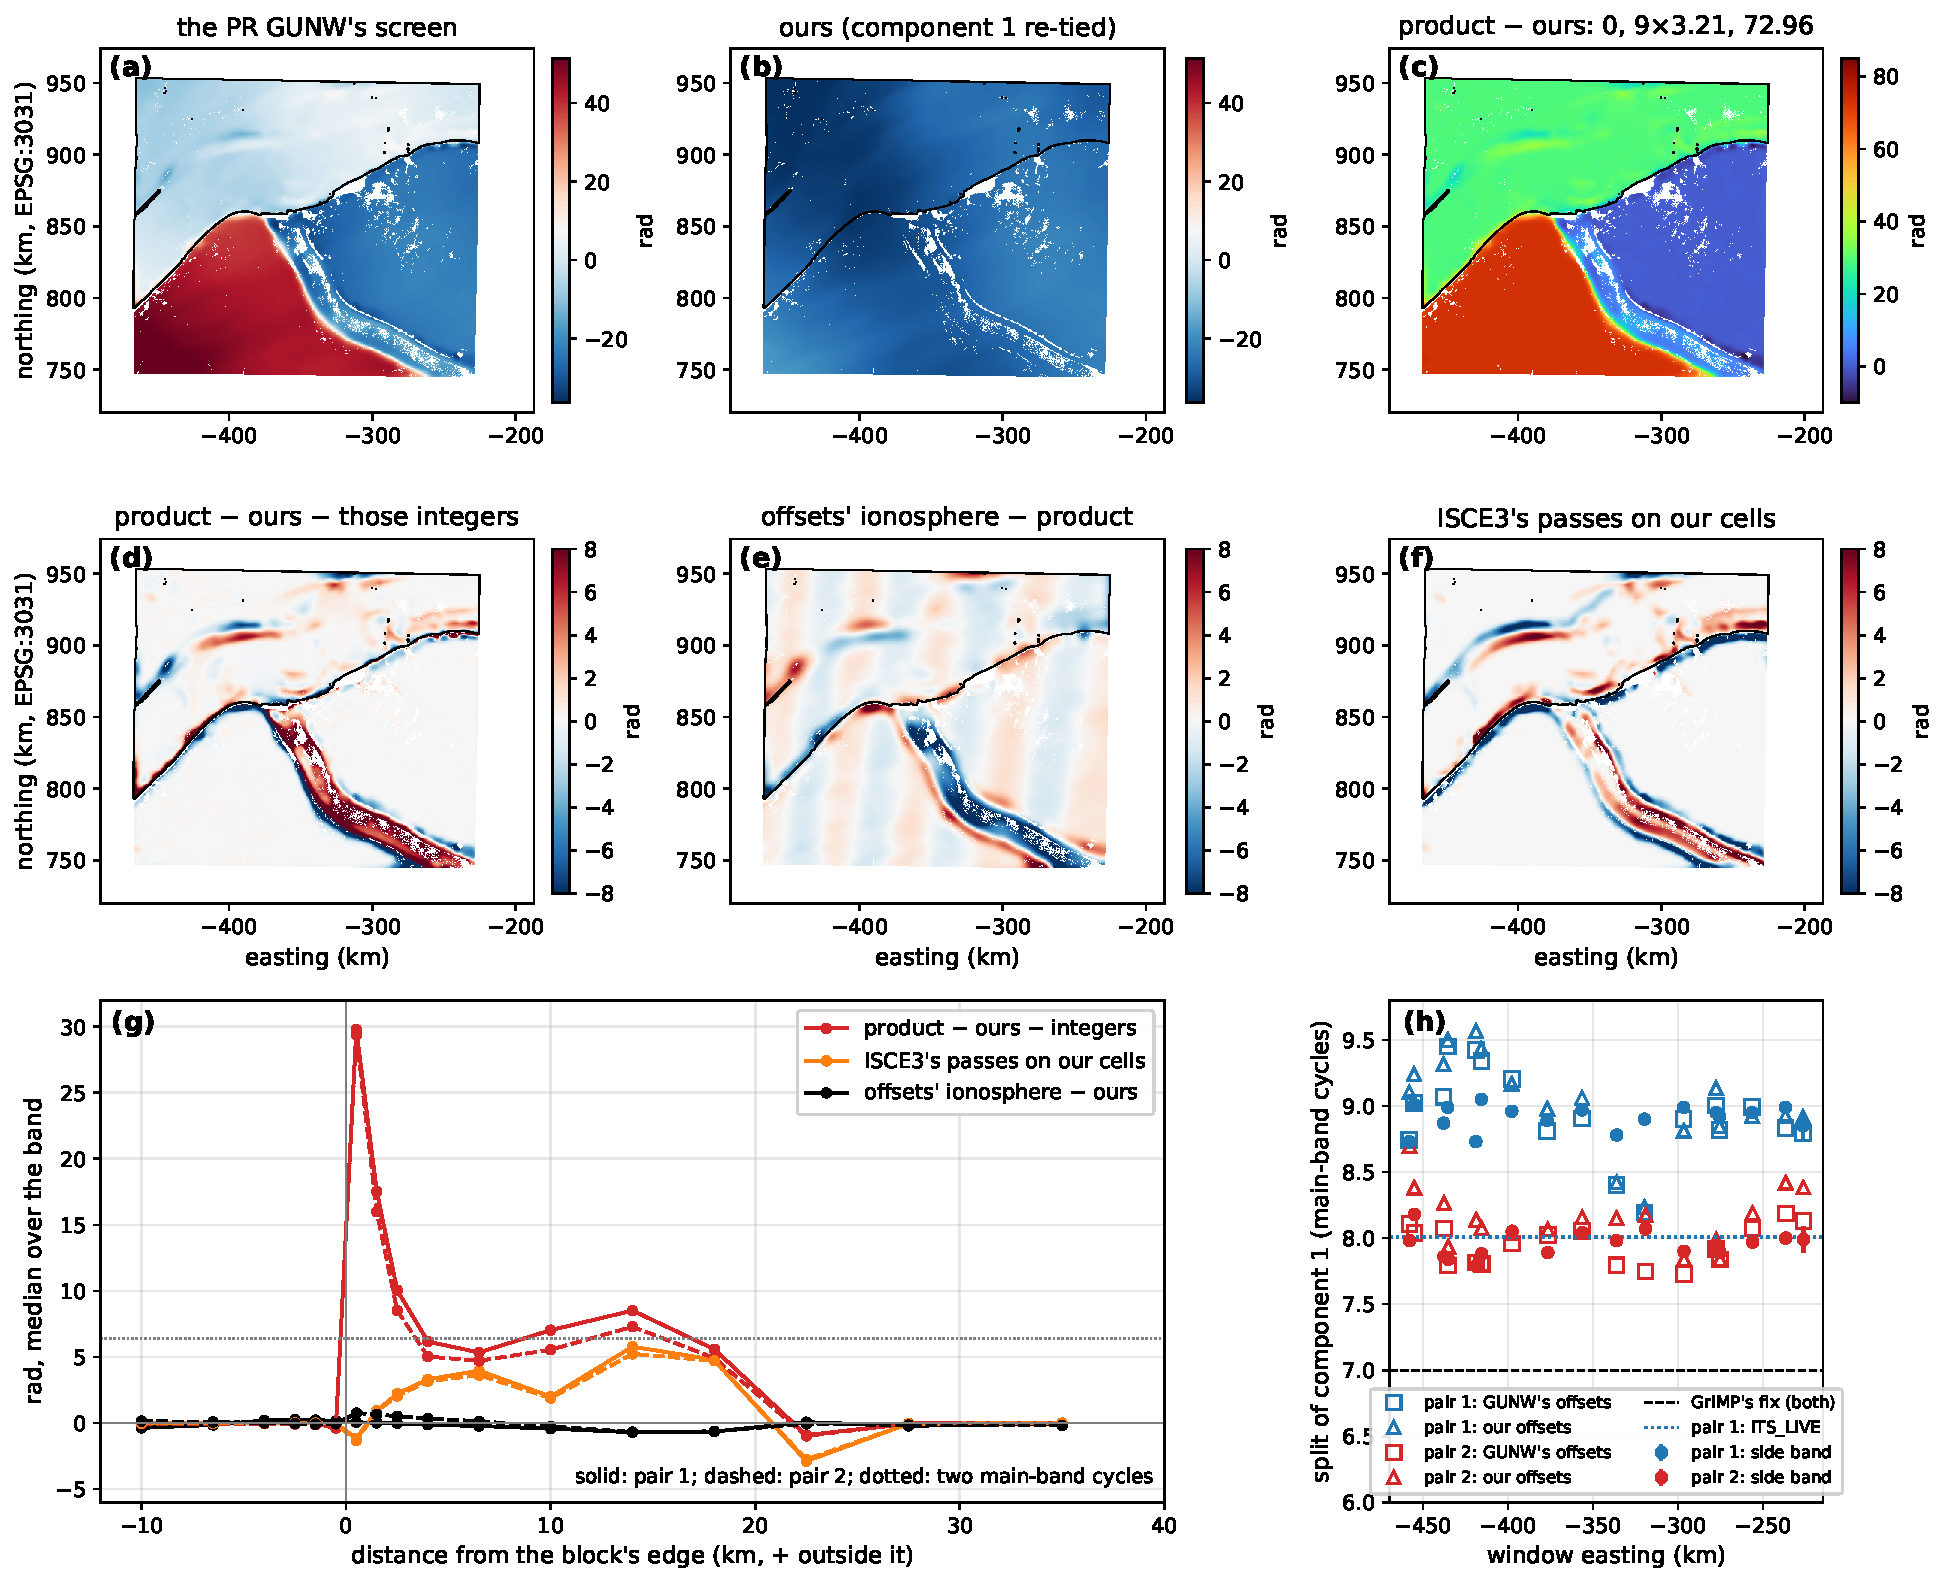
\includegraphics[width=\textwidth]{figures/fig_antarctica}
\caption{The Antarctic pair 19--31 August; pair 2 is alike (Table~\ref{tab:antarctica}).
(a) The PR GUNW's ionospheric screen. Black is the boundary between its connected components.
(b) Ours, with component 1 re-tied by the side band.
(c) Their difference takes three levels: 0; 9 main-band cycles (28.9\,rad) on component 1; and one cycle of the double
difference (73.0\,rad) over the block.
(d) What is left after those integers: the block's smeared edge, and the tributary's trunk.
(e) The offsets' ionosphere minus the product's screen, its integers repaired. The stripes are the offsets' own.
(f) What ISCE3's two correction passes add on our cells.
(g) Across the block's edge, median in bands parallel to it: the product's leftover, the passes on our cells, and the
offsets' ionosphere minus ours.
(h) The split of component 1 in the side band's 17 windows, by the side band and by the range offsets (the GUNW's and
our own), beside GrIMP's fix and ITS\_LIVE's reading.}
\label{fig:antarctica}
\end{figure}

\subsection{The product's screen is ours plus integers}
Product minus ours takes three levels (Fig.~\ref{fig:antarctica}c, Table~\ref{tab:antarctica}). Its baseline is the
densest $\pm5$\,rad window on component 2, because the block pulls that component's median.
\begin{itemize}
  \item On component 1 it is $+28.93$\,rad in pair 1 and $+25.69$\,rad in pair 2: 9.013 and 8.004 main-band cycles of
        3.21\,rad (robust sd 0.25 and 0.26). The product carries the main band's split between its components into its screen,
        as Table~\ref{tab:integers} says it must. Our tied screen does not step across the boundary: $-0.4$\,rad,
        2--8\,km either side, against the product's $+25.5$ and $+23.0$.
  \item Over a block of 11\,980 and 11\,304\,km$^2$ in component 2, between the component boundary and a tributary's
        western shear margin, it is $+73.00$ and $+72.92$\,rad in the block's core (robust sd 0.04): 1.0006 and 0.9995
        cycles of the double difference. This is the block that \citet{joughin2026nisarerrors} describe.
  \item Everywhere else it is 0.00\,rad (robust sd 0.07).
\end{itemize}
The block is the second mechanism of Section~\ref{sec:theory}. Decorrelated margins cut it off on both sides. The
non-dispersive phase steps across them by 167 and 120\,rad (3--6\,km either side, pair 1; pair 2 within 2\%), which puts
1.17 and 0.84 cycles into $\Delta$: more than $\pi$ across each gap. The product's unwrapping of $\Delta$ left the block
a cycle off both its neighbours. On our cells SNAPHU fails the same way, with the cycle on a different side: it puts
component 1 one cycle of $\Delta$ off, across the boundary where the step puts 1.06 cycles into $\Delta$. Ours unwraps
nothing that carries the flow.

\subsection{What is left after the integers}
After the integers, the screens still differ by more than 3\,rad over 5\,400 and 5\,078\,km$^2$
(Fig.~\ref{fig:antarctica}d). Two things make it (Fig.~\ref{fig:antarctica}g).
\begin{itemize}
  \item Within 3\,km outside the block's edge, the product is 17.7 and 16.4\,rad above ours (median). This is the
        product's filter smearing the block's 73\,rad step over a few kilometres, which no integer can repair.
  \item From 5 to 20\,km outside the block, over the tributary's trunk (1\,794 and 1\,820\,km$^2$), there is a plateau of
        6.50 and 5.44\,rad: 2.03 and 1.70 main-band cycles. The filter cannot smear that far.
\end{itemize}
The plateau is the first mechanism. We ran ISCE3's two correction passes (Section~\ref{sec:corrections}) on our cells,
with the main band tied. They move main-band cycles at 21\% of the cells, and over the plateau they raise the screen by
3.60 and 3.52\,rad (90th percentile 7.9). That is the product's place and sign, at about 60\% of its size
(Fig.~\ref{fig:antarctica}f).

Elsewhere the passes on our cells do more than the product shows: they are 18\,rad low where the product is 3\,rad low.
The passes ran on the product's own grid, which our cells do not reproduce, as on the Venezuela tracks
(Section~\ref{sec:nisar}). More than 5\,km from either integer step, the product's screen regresses on the 15\,km
high-pass of the non-dispersive phase at $-0.066$ ($r = -0.65$ and $-0.67$) in both pairs, and ours at $+0.002$ and
$+0.001$. That is the sign-flipped copy of Section~\ref{sec:intro}, here of the ice flow.

\subsection{Which screen is right over the fast ice}
The range offsets can tell. Phase advance and group delay have opposite signs, so $\phiA - k\rho_\mathrm{off}$ cancels
the flow and leaves twice the ionosphere, where $k = 4\pi\fA/c$ and $\rho_\mathrm{off}$ is the slant-range offset.
GrIMP's screen rests on the same physics \citep{joughin2026nisarerrors}. We use two sets of offsets. The GUNW's are
ISCE3's dense offsets (128-pixel windows every 75 pixels), culled, refilled and filtered for its rubbersheet. Our own come
from the same correlator ported to \texttt{nisar\_tools.roff} (64-pixel windows every 150 pixels), with only gross
outliers removed: those at the edge of the search, or more than 1\,m from the median of their $5\times5$
neighbourhood.

Smoothed over 3\,km, the offsets' ionosphere is calibrated on our screen where the two screens agree, as a slope plus a
plane. The slope is 2.01 and 1.83 with the GUNW's offsets, and 2.04 and 1.86 with ours, against 2 in theory. Where the
product departs, both sets follow our screen.
\begin{itemize}
  \item Where the product is more than 3\,rad above ours, the GUNW's offsets are $-0.28$ and $-0.32$\,rad from ours and
        $-5.60$ and $-4.91$\,rad from the product. Ours are $+0.11$ and $-0.20$ from ours and $-4.95$ and $-4.55$ from the
        product.
  \item Where the product is more than 3\,rad below ours, the GUNW's are $+0.34$ and $+0.27$ from ours and $+3.47$ and
        $+3.01$ from the product. Ours are $+0.26$ and $0.00$ from ours and $+3.31$ and $+2.73$ from the product.
\end{itemize}
(Table~\ref{tab:antarctica}; Fig.~\ref{fig:antarctica}e, g.) The product's departure does not scale with the unwrapped
phase ($R^2$ 0.03--0.04), so it is not a wrong frequency ratio.

\subsection{The components' split, three ways}
The side band ties component 1 at 8.95 cycles in pair 1 and 7.97 in pair 2. Each is the median of 17 windows along the
boundary, with a spread of 0.09. The range offsets, read the same way (a plane and a step in 30\,km windows at the same
17 places, using pixels 3--15\,km from the other component), give 8.90 and 7.96 with the GUNW's offsets, window by
window (Fig.~\ref{fig:antarctica}h). Our own offsets give 9.06 and 8.15 (spread 0.34 and 0.21).

Velocity maps read lower. ITS\_LIVE's version-2 mosaic \citep{gardner2018its,itslive2024v2}, on slow ice within 20\,km of
the boundary, reads 8.01 in pair 1. GrIMP's map reads the phase's step across the boundary as 7.5 cycles
\citep{joughin2026nisarerrors}. Component 2's side of the boundary is fast ice, so the nearest slow ice is across the
trunk, and a velocity map's error there enters the tie whole. The split is therefore 9 and 8 cycles, and GrIMP's $-7$
leaves component 1 two and one cycles off in the unwrapped phase. A residual metric that removes each component's
median cannot show that.

This boundary is also the control that Section~\ref{sec:sbtie} lacked. The non-dispersive phase steps across it by
74--188\,rad (median 162\,rad, 3.1\,m of LOS), as much as across the Panama ruptures. There the side band agrees with a
tie that shares none of its assumptions, so a bias of the side band that grew with the step would show up here as a
cycle. This is one look direction, descending.

\subsection{How good each correction is}
Three measures score the corrected phase, $\phiA$ minus a screen (Table~\ref{tab:antarctica}). The first two need no
velocity map.

\paragraph{Against the offsets' ionosphere.} With the phase tied, $(\phiA - k\rho_\mathrm{off})/2$ is an ionosphere
estimate independent of both screens, and here nothing is calibrated on either. It and each screen are smoothed over
6\,km, and a median and a plane are removed per screen. Our screen then departs from it by 0.63 and 0.68\,rad rms
(1.2--1.3\,cm of LOS). The product's screen misses it by 18.9\,rad as delivered, mostly through its integers. Once they
are repaired it misses by 1.29 and 1.21\,rad, twice ours, from the trunk's plateau and the smeared block edges.

\paragraph{Pair consistency.} Both pairs span 12 days on one track, so for steady flow their corrected phases should
match. Pair 1 minus pair 2, with a median and a plane removed, leaves what the corrections missed, noise, and any change
in the flow; 6.6 million pixels are coherent in both. Uncorrected it is 3.94\,rad (robust 4.13), the ionosphere that
changed between the pairs. Both screens remove most of it: the product's leaves 1.30 (0.99), ours 1.02 (0.81).

This measure cannot see errors that repeat in both pairs, and the product's do: the same block, splits of 9 and 8
cycles, the same plateau. That is why the product scores nearly as well as ours here. (Its repaired version scores 2.70,
because the repair of the smeared block edges differs between the pairs.) Faint stripes remain under both screens. The
carrier error of \citet{joughin2026nisarerrors}, which no screen removes, is a candidate; we have not tested it.

\paragraph{Against a velocity synthetic.} We also computed \citet{joughin2026nisarerrors}'s own metric: the phase minus a synthetic interferogram, with each
component's median and a plane removed. The synthetic comes from ITS\_LIVE's 120\,m static mosaic, projected on the
GUNW's line of sight over 12 days, with surface-parallel vertical flow. Pixels need coherence above 0.3 and grounded ice.

The multi-year mosaic misses the fast trunks: the product's corrected phase regresses on it at 0.40 above 200\,m/yr.
So only slow ice ($<$50\,m/yr), where the slope is 0.998 and 0.994, is meaningful.
\begin{itemize}
  \item Our screen leaves 1.84\,rad there in both pairs (robust 1.22 and 1.21).
  \item The uncorrected phase leaves 3.50 and 2.09 (3.15 and 1.69).
  \item The product's screen leaves 15.2 and 15.1 (14.2 and 14.1).
  \item Repairing the product's integers brings it to 4.0 (1.4); the smear and the trunk's cycles remain.
\end{itemize}
These numbers cannot be compared with those of \citet{joughin2026nisarerrors}, which use GrIMP's velocity map over all
ice with coherence above 0.3.

\subsection{What the Antarctic pairs show}
Each way the integers can go wrong in Section~\ref{sec:theory} appears in these products, in whole cycles.
\begin{itemize}
  \item The main band's split between its components is carried at 3.21\,rad per cycle: 9 and 8 cycles.
  \item One cycle of the double difference was unwrapped across decorrelated margins: 73\,rad over 12\,000\,km$^2$.
  \item The correction passes moved about two main-band cycles over a fast trunk.
\end{itemize}
None of this needs an earthquake: a glacier's shear margins are enough. The reordered estimate avoids the second and
third by construction, and the side band, checked here by the range offsets, repairs the first. Wherever the two can be
compared, our screen then agrees with the offsets' ionosphere to a few tenths of a radian.
